\documentclass[a4paper,11pt]{report}
%\documentclass[dvips]{seminar}
\usepackage{pslatex}
\usepackage{graphicx}
\usepackage[usenames]{color}
\pagestyle{plain}
%\textwidth=26cm
%\textheight=19.0cm

\begin{document}
%\setlength{\oddsidemargin}{-.01cm}
%\setlength{\topmargin}{-2.cm}

\begin{center} \huge
{\bf \color{red} BigDFT User Manual}
\end{center}

\large
\begin{itemize}
\item Stefan.Goedecker@unibas.ch \\
http://www.unibas.ch/comphys/comphys \\
\item Luigi.Genovese@esrf.fr \\
\item Damien.Caliste@cea.fr
\end{itemize}
\normalsize
\tableofcontents

\chapter{Installing BigDFT}

The compilation and installation of BigDFT relies on the GNU standard building chain: 'configure', 'make', 'make install'. BigDFT can be used an independent program (as described in this manual), or as a library, to be embeded in other softwares, like inside ABINIT.

\section{Building the executables}

\subsection{Configure}
BigDFT build system is based on standard GNU autotools. The end
user does not need to have the Autotools package installed on his
computer, the \texttt{configure} script provided in BigDFT package
will to the job to create the \texttt{Makefile} and set the
options, like the optimisation level, the associated libraries to link
with...

After the package has been untared, the sources should be configured, depending on the system we want to run on. Thanks to the autotools, it is possible to generate several builds from the same source tree. It is adviced to create a compilation directory, either inside or outside the source tree. Lets call this directory \texttt{compile-gfortran} for instance. One starts the configure from there \texttt{'source tree path'/configure}.

The following modularities during compilation are available:
\begin{itemize}
  \item \texttt{--disable-mpi}: force not to use MPI during build. By default the configure will try to detect if the compiler has some native MPI capabilities. If not MPI will be automatically disabled.
  \item \texttt{--enable-cuda-gpu}: compile the CUDA parts to run on NVidia GPUs. This options requires to add some other one to find the CUDA environnement, see the \texttt{--with} options later.
\end{itemize}

One can tune the compilation environnement using the following options:
\begin{itemize}
  \item \texttt{--with-cuda-path}: give the path to the NVidia Cuda tools (default is \texttt{/usr/local/cuda}).
  \item \texttt{--with-cuda-cflags}: specify the flags for the NVidia Cuda Compiler.
  \item \texttt{--with-ext-linalg}: Give the name of the libraries replacing Blas and Lapack (default = none specified). Use the -l before the name(s).
  \item \texttt{--with-ext-linalg-path}: Give the path of the other linear algebra libraries (default = \texttt{-L/usr/lib}). Use the -L before the path(es).
  \item \texttt{FC}: Specify the compiler.
  \item \texttt{FCFLAGS}: Specify the flags, like the
optimisation flags, to pass to the compiler (default are \texttt{-g
-O2} for GNU compilers).
  \item \texttt{--prefix=DIR}: Specify your installation directory (\texttt{/usr/local} is default).
\end{itemize}

A example of compilation using the MKL from Intel instead of basic Blas and Lapack installation:\\
\texttt{../configure --with-ext-linalg="-lmkl\_ia32 -lmkl\_lapack"\\
   --with-ext-linalg-path="-L/opt/intel/mkl72/lib/32"\\
   --prefix=/home/caliste/usr FC=ifort}

An other example, compiling CUDA parts:\\
\texttt{../../sources/bigdft-1.3.0-dev/configure\\
  FC=mpif90 FCFLAGS="-O2  -assume 2underscores"\\
  CC=icc CXX=icc CXXFLAGS="-O2  -I/applications/cuda-2.2/include/"\\
  CFLAGS="-O2  -I/applications/cuda-2.2/include/"\\
  --with-ext-linalg="-L/applications/intel/mkl/10.1.1.019/lib/em64t\\
                     -lmkl\_scalapack\_lp64 -lmkl\_blacs\_intelmpi20\_lp64\\
                     -lmkl\_intel\_lp64 -lmkl\_lapack -lmkl\_sequential -lmkl\_core"\\
  --enable-cuda-gpu --with-cuda-path=/applications/cuda-2.2}

\subsection{Make}
Make the package and create the 'cluster' executable, issuing \texttt{make}. The GNU option \texttt{-j$n$} is working with whatever value of $n$ (tested up to 16).

\subsection{Install}
To install the package, issue \texttt{make install}. It will copy all files to the specified prefix (see configure).

\subsection{Clean}
Clean the source tree of the 'make' action by \texttt{make clean}.

\section{Building a library}
To avoid to create the binary executable,
use \texttt{--disable--build-binary} option.

\chapter{Structure of the BigDFT code}
\noindent
The main subroutine of the BigDFT package is the \texttt{call\_bigdft} routine. For a given set of input coordinates 
an input parameters it returns the total energy and the forces actiing on the nuclei. The \texttt{BigDFT.f90} main program 
calls the \texttt{call\_bigdft} routine and can also do a geometry optimization by calling the geopt routine (which in turn calls 
again \texttt{call\_bigdft}). For other standard applications other main programs exist.
At present main programs to do a vibrational analysis, saddle point search and global optimization have been developed.
Users are however encouraged to write their own main programs for specific applications. 
\section{The basis set}
The maximally symmetric Daubechies family of degree 16 is used to represent 
the Kohn-Sham orbitals. The two fundamental functions of this family, 
the scaling function $\phi$ and the wavelet $\psi$ are shown in Fig. \ref{sym_16} 
for the one-dimensional case.
To form a basis set these functions have to be centered on the nodes of a regular grid.
\begin{figure}[ht]
\begin{center}
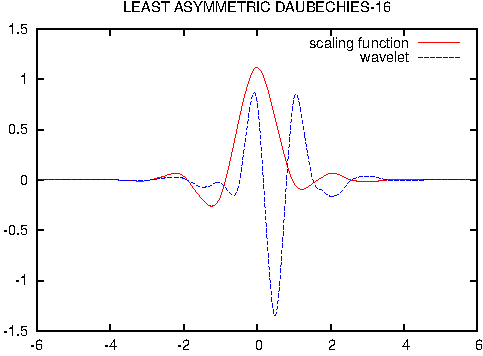
\includegraphics[width=\textwidth]{sym_16.pdf}
\end{center}
\label{sym_16}
\caption{Daubechies Scaling Function and Wavelet of order 16}
\end{figure}
\section{Wavelet basis sets in three dimensions}
A 3-dim wavelet basis is made by products of 1-dim functions.
 {\color{red} 1  scaling function } and {\color{blue} 7 wavelets } 
can be centered on the nodes (i,j,k) of a regular 3-dim cartesian grid.
They all are products of 1-dim scaling functions and wavelets
\begin{eqnarray*}
 {\color{red} \phi_{i,j,k}(x,y,z) }  & = & \phi(x-i) \phi(y-j) \phi(z-k)   \\
 {\color{blue} \psi^1_{i,j,k}(x,y,z) } & = & \phi(x-i) \phi(y-j) \psi(z-k)  \\
 {\color{blue} \psi^2_{i,j,k}(x,y,z) } & = & \phi(x-i) \psi(y-j) \phi(z-k)  \\
 {\color{blue} \psi^3_{i,j,k}(x,y,z) } & = & \phi(x-i) \psi(y-j) \psi(z-k)  \\
 {\color{blue} \psi^4_{i,j,k}(x,y,z) } & = & \psi(x-i) \phi(y-j) \phi(z-k)  \\
 {\color{blue} \psi^5_{i,j,k}(x,y,z) } & = & \psi(x-i) \phi(y-j) \psi(z-k)  \\
 {\color{blue} \psi^6_{i,j,k}(x,y,z) } & = & \psi(x-i) \psi(y-j) \phi(z-k)  \\
 {\color{blue} \psi^7_{i,j,k}(x,y,z) } & = & \psi(x-i) \psi(y-j) \psi(z-k)  \\
\end{eqnarray*}
If a grid point carries the 7 {\color{blue} wavelets} in addition to the {\color{red} scaling function} it belongs 
to the high resolution region. In the low resolution region a grid point carries only 
a single {\color{red} scaling function}. In the high resolution region the resolution is doubled 
in each diretion with respect to the low resolution region. The grid spacing is specified by the parameters
{\bf hgridx}, {\bf hgridy}, {\bf hgridz}. The low resolution region is constructed in the following way. Around each 
atom one draws a sphere whose radi are the 'size of the atom' times the parameter {\bf crmult}. All the grid 
points being contained in the union of all these spheres form the low resolution region. The high resolution is 
constructed in a similar way. One draws spheres whose radii are the 'size of the bonding region' times the 
parameter {\bf frmult} around each atom.  All the grid points being contained in the union of all these spheres 
form the high resolution region. Default values for the 'size of the atom' and  the 'size of the bonding region' 
are contained in the package. The user can however chose different values and these values can be specified by 
adding a additional line at the end of the pseudopotentila parameter files which contains first the altenative 
values of {\bf crmult} and then {\bf frmult}. The grid can be visualized by calling the 'memguess' program 
with the the keywords {\bf output\_grid}=1 in the input file. The output file 'grid.xyz' contains the atomic positions and in addition 
the grid points which denoted by 'g' if the are in the coarse region and by 'G' if they are in the fine region. 
Whereas the total number of basis functions is nearly independent of the orientation of the molecule, the size of some 
work arrays depends on the orientation. When the memguess routine is called with the option {\bf optimise} = .true., it will rotate 
a molecule that will be calculated with free boundary conditions in such a way that the simulation cell size and 
hence the size of the work arrays are as small as 
possible. The rotated output is written in the file posout\_000.xyz.

\begin{figure}[h]             % produce figure
\begin{center}
\begin{tabular}{cc}
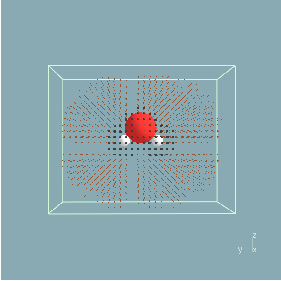
\includegraphics[width=0.4\textwidth]{grid100.pdf} &
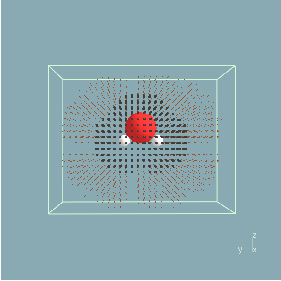
\includegraphics[width=0.4\textwidth]{grid200.pdf} \\
frmult=8 crmult=4 hgrid=.5 & frmult=12 crmult=4 hgrid=.5 \\
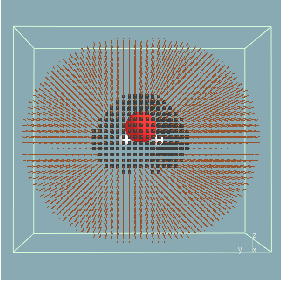
\includegraphics[width=0.4\textwidth]{grid300.pdf} &
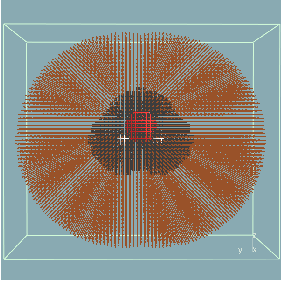
\includegraphics[width=0.4\textwidth]{grid400.pdf} \\
frmult=12 crmult=6 hgrid=.5 & frmult=12 crmult=6 hgrid=.3
\end{tabular}
\end{center}
\label{grids}
\caption{Illustration of the grid and its parameters}
\end{figure}

\section{Input/Output files for atomic coordinates } 
By default the atomic input coordinates are in the file 'posinp.xyz'. If the same operation (e.g. geometry optimization) 
has to be done for several structures one can also give a list of input files whose names (without the .xyz extension) 
have to be contained in a file 'list\_posinp'. The first line in the 'list\_posinp' file has to be the number of input 
files and each consecutive line contains then one filename. 
All the input and output files for atomic coordinates are in the .xyz format, i.e they can be visualized with any 
standard visualization package and in particular with V\_sim. The first line contains the number of atoms 
and then the units, which are specified by 'atomic', 'atomicd0' or 'bohr' if atomic units are used or by 
'angstroem' or 'angstroemd0' if Angstroem are used. 'd0' formats (e24.17) garantuee that not a single bit is 
lost during write and read of the numbers. 
The second line contains the boundary conditions specified by the keywords 'free' for free boundary 
conditions, 'periodic' for periodic boundary conditions or 'surface' for surface boundary conditions
where the x and z direction have periodic boundary conditions and the y direction free boundary conditions. 
The keywords 'periodic and 'surface' have to be followed by 3 real numbers giving the length of the 
orthorombic periodic cell. In the case of surface boundary condition the second of these numbers is ignored. 
The following lines contain the name of the chemical element followed by the 3 cartesian coordinates. 
Chemical elements are identified by their pseudopotential. If a element is for instance denoted by 
'Si' the element will be described by the file 'psppar.Si' which has to be present in the working directory 
of the BigDFT.run. A silicon atom could however also be denoted by 'Si\_lda' if there is file 'psppar.Si\_lda.
BigDFT supports the GTH and HGH pseudopotentials in the format which can be downloaded from the ABINIT website
(www.abinit.org). The 3 cartesian coordinates can be followed by optional additional information.
LUIGI PLEASE CHECK THIS PART:
In the case of spin-polarized calculation the polarization in the region around the atom can 
be given by an integer. In addition the charge in the region around the atom can be specified.
Finally it can be specified if the atom is fully or partially fixed during a geometry optimization.
'F' stands for completely frozen, 'FXZ' if the atom can only move along the y axis and 'FY' if the atom 
can only move in the XY plane. Below are some examples:

This hydrogen atom is frozen during the geometry optimization
\begin{verbatim}
  H  1.2  3.4  5.6   f
\end{verbatim}

This hydrogen atom has a spin up poarization
\begin{verbatim}
  H  1.2  3.4  5.6   1
\end{verbatim}

This chlorine atom has an additional electron and no spin polarization
\begin{verbatim}
  Cl  1.2  3.4  5.6   0  -1.
\end{verbatim}

Same as above, but also frozen
\begin{verbatim}
  Cl  1.2  3.4  5.6   0  -1.   f
\end{verbatim}

\pagebreak
\begin{center} \large
{ \bf The input file input.memguess}
\end{center}
Before running BigDFT it is recommended to run the memguess routine. If it runs correctly all input files are available 
(this routine needs a posinp.xyz and does not accept a list\_posinp file). It then allows to estimate the required memory and to 
find an optimal number of MPI processes for a parallel run. For good load balancing each MPI process should roughly treat the same number 
of orbitals. The memguess program prints out the number of orbitals and how many orbitals are treated by each MPI process. 
On a parallel machine with a high performance interconnect network on can choose the number of MPI processes {\bf nproc} equal 
to the number of occupied orbitals, i.e. each MPI process treats one orbital. On machines with slower networks each MPI process should 
have at least 2 to 4 orbitals. 
\begin{itemize}
\item {\bf nproc}: Number of MPI processes
\item {\bf optimise}: if =.true. the molecule will be rotated such that the size of the workarrays is minimal
\item {\bf output\_grid}: if =1 the file grid.xyz will be generated, =0 otherwise
\item {\bf GPUtest}: if =.true. perform the test with GPU
\end{itemize}


\section{The input file input.dft}
This file contains all the parameters required for a single wavefunction calculations
\begin{itemize}
\item {\bf hgridx},{\bf hgridy},{\bf hgridz}: The grid spacing of the cartesian grid. As 
        described above the nodes of this grid serve as the centers for the scaling function/ wavelet basis. 
       Values are in most cases between .3 and .6

\item {\bf crmult}, {\bf frmult} Coarse Region Multiplier and Fine Region Multiplier which serve to determine the radius
      radius for the low/high resolution sphere around the atom. 
      Values are typically of the order of 5 for {\bf crmult} and of the order of 10 for  {\bf frmult}.
\item {\bf ixc}: integer specifying which exchange correlation functional will be used. The Abinit conventions are 
      used and detailed information can be found on the Abinit Web page 
      (http://www.abinit.org/documentation/helpfiles/for-v5.8/input\_variables/varbas.html\#ixc). 
       Here is only a short summary of some widely used functionals:
      \begin{itemize}
      \item  1: Pade LDA from Abinit XC library
      \item  11: PBE from Abinit XC library
      \item -020: Pade LDA from libXC
      \item -101130  PBE from  libXC
      \item -116133 PBEsol from libXC
      \end{itemize}
\item {\bf ncharge}, {\bf elecfield}: total charge of the system and constant electric field along the y direction in units of Ha/bohr. 
      A positive {\bf ncharge} means that electrons are taken away.
\item {\bf nspin}, {\bf mpol}: nspin=1: closed shaell system without spin polarization, nspin=2: spin polarized 
      system, nspin=4: non-collinear magnetic system
\item {\bf gnrm\_cv} convergence criterion for the wavefunction optimization (norm of the gradient).
      Reasonable values are in most cases between 1.d-4 and 1.d-5
\item {\bf itermax}, {\bf nrepmax}: Maximum number of gradient evaluations for a single cycle in a wavefunction optimization 
      and maximum number of cycles. At the end of each cycle a subspace diagonalization is done which helps 
in cases where one has near degenercy between the homo and lumo orbitals. 50 and 2 are usually sufficient.
\item {\bf ncong}, {\bf idsx}: ncong gives the number of iterations in the solution of the preconditioning equation.
      For free boundary conditions 5 is a good value for periodic boundary condition 0 to 2 is sufficient and for 
      periodic boundary conditions ??. Large values of {\bf ncong} lead to a smaller number of iterations in 
      the wavefunction optimization, but each iteration is more costly. So a optimal compromise value has to be found.
      {\bf idsx} gives the history length of the DIIS convergence acceleration in the wavefunction optimization.
      6 is usually a good value for fast convergence. In case of convergence problems it can be advantageous 
      to switch off DIIS by setting {\bf idsx} =0. The memory requirements grow considerably with large values of 
      {\bf idsx}. If memory is the limiting factor one has to choose {\bf idsx} smaller than the value which gives 
      the fastest convergence. The memguess tool can be used to predict the emeory requirements for different choices 
      of  {\bf idsx}.
\item {\bf dispersion}:  A non-zero values activates an  empirical add-on treatment of dispersion effects.
       the values 1,2 and 3 specify different switching on functions using the convention of 
       Q. Hill and C.-K. Skylaris.  Proc. R. Soc. A 465  (2009) 669
\item  Putting the keyword "CUDAGPU" in this line will activate the use of Cuda versions of various subroutines.
       a GPU.config file is needed in this case. 
\item {\bf InputPsiId }, {\bf  output\_wf},  {\bf output\_density }: 
       {\bf InputPsiId } specifies how the input guess wavefunction is generated
      \begin{itemize}
       \item {\bf InputPsiId } -2 : Random numbers are used as input guess. This is of course a poor input guess which will 
                                    need many iterations of the wavefunction oprimization and might even lead to divergencies.
       \item {\bf InputPsiId } -1 : The input wavefunction is imported from the CP2K code which uses Gaussians
       \item {\bf InputPsiId } =0 : A subspace diagonalization in a minimal atomic basis set is used. This input guess 
                                    should be used in general if one starts a new calculation. 
       \item {\bf InputPsiId } =1 : The previously calculated wavefunctions (for instance from the previous 
                                    geometry optimization step) are used as input guess. Setting {\bf InputPsiId } to 
                                    this value does only make sense from within a main program where call\_cluster was 
                                    called previously. The old wavefunction is passed to the new call via the data structure 'restart'
       \item {\bf InputPsiId } =2 : The input wavefunction is read from the 'wavefunction.*' files which contain all the 
                                    scaling function and wavelet coefficients. In case some parameters such as {\bf hgridx} 
                                    or {\bf crmult} have changed, compared to the previous run, the wavefunctions will be 
                                    transformed to the new parameter set.
       \item {\bf InputPsiId } =11: restart with Gaussian approximation contained in the 'restart' data structure.
       \item {\bf InputPsiId } =12: The input wavefunction is read from the 'wave.gaus'  file, which contains an 
                                    approximation in a minimal Gaussian basis set of the previously calculated wavefunctions.
       \item {\bf output\_wf} : If .true. the output wavefunction is written at the end of the wavefunction optimization 
                               into files. If {\bf InputPsiId } was greater than 10 the wavefunction will be written 
                               in the Gaussian approximation into  a single 'wavefunctions.gau' file otherwise into 
                               'wavefunction.*' files. Writing a  'wavefunction.*' file for each orbital can take a considerable 
                               amount of time and disk space. 
       \item {\bf output\_density} = 0, no output density is written
       \item {\bf output\_density} = 1, output electronic density is written in the .pot format of V\_sim into the file 'electronic\_density.pot'
       \item {\bf output\_density} = -1, same as  {\bf output\_density} = 1, but using .cube format: electronic\_density.cube
       \item {\bf output\_density} = 2, in addition to the electronic charge density the following files are written:
                                  'ionic\_potential.pot', 'local\_potential.pot', 'hartree\_potential.pot'.
       \item {\bf output\_density} = -2, same as {\bf output\_density} = 2, but all files are written in the .cube format
      \end{itemize}
\item {\bf calc\_tail} , {\bf rbuf}, {\bf ncongt}:  Far reaching tails of the wavefunctions decaying into the vacuum are  
                                      added in a perturbative treatment if the variable {\bf calc\_tail} is set to .true.. 
                                      This allows to do a calculation with some moderate 
                                      value of {\bf crmult} and then to extrapolate to the limit of large  {\bf crmult}. 
                                      This procedure is not variational and gives too low energies. The true energy is 
                                      in between the two energies and in general much closer to the extrapolated energy. 
                                      This procedure can also be used to judge whether the chosen value of  {\bf crmult} is 
                                      large enough for a certain required precision. 
                                      {\bf rbuf} gives the amount by which the radii for the coarse resolution region 
                                      are increased in atomic units. {\bf ncongt} gives the number of iterations used 
                                      in the pertubation calculation. Reasonable values for {\bf ncongt} are around 30.  

\item {\bf nvirt}, {\bf  nplot}: Usually virtual (unoccupied) orbitals are not calculated since they are not needed for 
                                 the total energy and other physical properties of the electronic ground state. 
                                 Putting  {\bf nvirt} to a non-zero 
                                 value will result in the calculation of {\bf nvirt} virtual orbitals in a postprocessing 
                                 routine after the occupied orbitals have been calculated. {\bf nplot}  of these 
                                 orbitals will be written in the 'virtual.*.pot' files and {\bf nplot} (if that many exist) 
                                 of the highest occupied orbitals will be  written in the 'orbital.*.pot'file
                                 The Kohn Sham eigenvalues are written in the ordinary output file. 
 

\item {\bf iat\_absorber} x\_ray absorber treatment????
\item {\bf atom no., read\_ref\_den, correct\_offset, gnrm\_sw} vacancy?????
\item {\bf verbosity} : determines the amount of output from little (0) to detailed (2)
\end{itemize}

\section{The input file input.geopt}
If this file exists BigDFT will do a geometry optimization and the file contains all the required parameters

\begin{itemize}
\item {\bf geopt\_approach} : this character string specifies the method used for the geometry optimization.
       \begin{itemize}
       \item  \emph{VSSD}: Variable Stepsize Steepest Descent method
       \item  \emph{SDCG}: A combination od Stepest Descent and Conjugate Gradient
       \item  \emph{LBFGS}: Limited Memory BFGS
       \item  \emph{AB6MD}: The molecular dynamic routines from ABINIT 6
       \end{itemize}
\item  {\bf  ncount\_cluster\_x} : Maximum number of force evaluations to be used for the geometry optimization.
\item  {\bf frac\_fluct },{\bf forcemax } : Convergence criteria for the geometry optimization. The geometry optimization stops either 
                                           if the norm of any force acting on any atom in the system is smaller than {\bf forcemax } 
                                           or if the forces get noisy. Noise is present because of the underlying integration grid.
                                           The parameter {\bf frac\_fluct } specifies how small the forces should become 
                                           compared to the noise level to stop the geometry optimization. 1 is a reasonable parameter 
                                           for this parameter and it means that the geometry optimization will stop when the noise 
                                           in the forces is comparable to the forces themselves. For values of  {\bf frac\_fluct } 
                                           smaller than 1 one can under certain circumstances obtain better relaxed geometries but 
                                           one risks that the geometry optimization will not converge. In such a case one should 
                                           closely monitor the prgress of the geometry optimization by looking at the 'posout.*' 
                                           files which are written at each step of the geometry optimization and at the 'geopt.mon' file. 
\item  {\bf randdis } : This parameter allows to add random displacements with amplitude randdis to the atomic positions in the 
                        input file posinp. This can for instance be useful to break degeneracies (which would lead to 
                        convergence problems in the wavefunction optimization) in highly symmetric structures.
\item  {\bf betax } : This is the stepsize for the geometry optimization. This stepsize is system dependent and it has therefore to be 
                      determined for each system. If the VSSD method is used one can start with a small stepsize of around 1 and 
                      VSSD will suggest than a better value for {\bf betax } in the last line of the 'geopt.mon' file. 
                      Whether the stepsize is correct can also be seen from the 'geopt.mon' output of the SDCG method. In this 
                      case the average stepsize in terms of betax should be around 4 (after a brief initial period where it is around 8).
                      In constrast to the SDCG method the LBFGS method is not very sensitive to the correct stepsize but nevertheless 
                      one should try to find reasonable values also in this case.
\item  \textbf{ionmov} : in case of {\bf geopt\_approach = AB6MD}, the {\bf betax } line should be replaced by this one. It contains an integer value as described in the ABINIT manual. Possible values are:
                         \begin{itemize}
                         \item 6: simple velocity-Verlet molecular dynamic.
                         \item 7: quenched molecular dynamic, when the scalar product force / velocity becomes negative, the velocity is set to zero. The force criterion is tested at each step.
                         \item 8: Nose-Hoover thermostat.
                         \item 9: Langevin dynamic (adding a friction force and a gaussian random force on atoms).
                         \item 12: Isokinetic ensemble molecular dynamics. The equation of motion of the ions in contact with a thermostat are solved with the algorithm proposed by Zhang [J. Chem. Phys. 106, 6102 (1997)], as worked out by Minary et al [J. Chem. Phys. 188, 2510 (2003)]. The conservation of the kinetic energy is obtained within machine precision, at each step.
                         \item 13: Iosthermal/isenthalpic ensemble. The equation of motion of the ions in contact with a thermostat and a barostat are solved with the algorithm proposed by Martyna, Tuckermann Tobias and Klein [Mol. Phys., 1996, p. 1117].
                         \end{itemize}
\item  \textbf{dtion} : the time step for molecular dynamic, in atomic time units. One atomic time unit is 2.418884e-17 seconds, which is the value of Planck's constant in hartree*sec. The following lines depend on the choosen value for \textbf{ionmov}.
\item  if \textbf{ionmov = 6} : one line containing the initial temperature in kelvin. If negative, the initial velocities are all zero. If positive, random speeds are chosen to match the given temperature (NOT implemented yet!).
\item  if \textbf{ionmov $>$ 7} : one line containing two temperatures in kelvin. When different, the temperature is linearly change at each geometry step to go from the first value to the second.
\item  if \textbf{ionmov = 8} : one additionnal line containing the thermostat inertia coefficient for Nose-Hoover dynamic.
\item  if \textbf{ionmov = 9} : two additionnal lines containing first the friction coefficient and then a value in bohr corresponding at a distance where the atoms can bounce on (see the ABINIT documentation for further details).
\item  if \textbf{ionmov = 13} : several additionnal lines containing first the number of thermostats in the chain of thermostats. Then a line with the mass of each thermostat in the chain. And finally a line with two values for the barostat mass, depending on optcell value (NOT implemented yet).


\end{itemize}

\section{The input file input.kpt}
This file is used to specify a set of $k$ points. If this file does not exist, only the $\Gamma$ point will be used. The $k$ point generation relies on the ABINIT implementation. This files contains the following information:
\begin{itemize}
  \item  \textbf{kptopt}: this character string specifies the method used to generate the $k$ point mesh.
       \begin{itemize}
       \item  \emph{auto}: automatic generation is used, based on the $k$ point density we whish in Fourrier space, taking into account the symmetries of the system.
       \item  \emph{MPgrid}: a Monkhorst-Pack grid, using only the special $k$ points, taking into account the symmetries of the system.
       \item  \emph{manual}: a manual set of $k$ points.
       \end{itemize}
       The following lines depend on the choice of \textbf{kptopt}.
  \item  if \textbf{kptopt = 'auto'}: one additionnal line containing a real space length \textbf{kptrlen}. BigDFT will automatically generate a large set of possible $k$ point grids, and select among this set, the grids that give a length of smallest vector LARGER than \textbf{kptrlen}, and among these grids, the one that, reduces to the smallest number of $k$ points.
  \item  if \textbf{kptopt = 'MPgrid'}: several additionnal lines. The first line should contains three integers describing the mesh of Monkhorst-Pack grid in reciprocal space. The second line contains one integer \textbf{nshiftk} that give the number of shift one would ike to apply to the MMP grid to obtain the final $k$ point mesh. Then the file contains \textbf{nshiftk} lines with three real numbers each, giving the shift to apply in reciprocal space.
  \item  if \textbf{kptopt = 'manual'}: several additionnal lines. The first contains \textbf{nkpt}, an integer giving the number of manually defined $k$ points. Then \textbf{nkpt} lines follow, whith four real values each, the three firsts being the coordinates in reciprocal space (in $[0;0.5]$) and the fourth bing the weigth. If the sum of all weigths does not equal to one, weight values are renormalised.
\end{itemize}

\chapter{ Running Bigdft executables}

\section{Doing a single point or a geometry optimization: \texttt{cluster}}
The MPI version is executed on most machines with the mpirun command followed by the name of the executable which is 
cluster in our case.
The treatment of each orbital can be speeded up by using the mixed MPI/OpenMP implementation 
where each MPI processes uses several OpenMP threads to do the calculations for its orbitals faster. 
The OpenMp is simply activated by compiling the program with an OpenMP flag and by specifying the number of OpenMP threats by
export OMP\_NUM\_THREADS=4 if 4 threads are for instance desired.

\noindent
The Bigdft program monitors during a run the memory utilization and the time spent in various subroutines. Detailed information 
is written in the files malloc.prc and time.prc. At the end the program checks whether the number of deallocations was equal 
to the number of allocations and whether the total memory went back to zero. If this should not be the case please send a bug report to the develpers of BigDFT.

\section{Doing a path minimization: \texttt{NEB}}
A NEB implementation is present in the BigDFT package, thanks to the initial routines provided by Carlos Sbraccia. This implementation is launched with the help of the \texttt{NEB} executable. This program is responsible for initialising the path from the two minima and then to run the path minimisation, using BigDFT to compute the forces. Each replica is launched by an instance of \texttt{cluster} and not in the same program \texttt{NEB}. This allow to run the NEB algorithm on a super computer with a queue system. Each replica going separatly in the queue. The process of running the different \texttt{cluster} instances, in different directories and wait for their completions is done by two shell scripts: \texttt{NEB\_driver.sh} and \texttt{NEB\_include.sh}. The first one is very generic and should not be touched by users. It is provided in the \texttt{src/} directory of the package. The second one must be adapted by users to suit to their running machine. One example one is provided in the \texttt{tests/NEB/} directory of the package.

The \texttt{NEB} executable can be run from everywhere but \texttt{NEB\_driver.sh} and \texttt{NEB\_include.sh} must be in the same directory. It takes arguments from the command line, using a redirection from a file is good practice. See the \texttt{tests/NEB} directory of the package:
\begin{center}
  \texttt{./NEB < input}
\end{center}
The file \texttt{input} contains a list of variables relevant to the NEB algorithm. Some of them are explained here:
\begin{itemize}
  \item \texttt{scratch\_dir} is where the \texttt{NEB\_driver.sh} script will create the directories where to run the \texttt{cluster} instances. It is usually on a local disk.
  \item \texttt{job\_name} a name that will be used to named all generated files and directories.
  \item \texttt{climbing} when set to \texttt{.TRUE.}, the highest replica follow opposite parallel forces in addition to the usual perpendicular ones.
  \item \texttt{optimization} when set to \texttt{.TRUE.}, try to optimize the geometry of the first and last replicas (if not local minima already).
  \item \texttt{minimization\_scheme} possible values are 'steepest\_descent', 'fletcher-reeves', 'polak-ribiere', 'quick-min', 'damped-verlet' and 'sim-annealing'.
  \item \texttt{tolerence} is a criterion not to take into account in the list of moving atoms the ones that move less than this value between the first and the last replica.
  \item \texttt{convergence} is the stop criterion on perpendicular forces, in eV/\AA.
  \item \texttt{num\_of\_images} is the number of desired replicas.
  \item \texttt{*\_config} the file describing the first and the last replica (in BigDFT 1.3, the file extension .xyz must be omitted).
\end{itemize}

At each NEB iteration, the driver script is runned. It creates the directories for forces calculations if needed, create the input files using the include script, run the jobs, grep the energy and the forces and return. The script file \texttt{NEB\_include.sh} must contain the following shell functions:
\begin{itemize}
  \item \texttt{init\_jobs()}, run once after directory creation. It can be used.
  \item \texttt{finalise\_jobs()}, run once after all jobs have finished.
  \item \texttt{wait\_jobs()}, run each time the script poll all replicas for completion.
  \item \texttt{make\_input()}, run once in each scratch directories to create the posinp.xyz file from the NEB restart file and the initial ones.
  \item \texttt{run\_job()}, run once in each scratch directories to start the force calculations. In the example, it runs the replicas directly on the host machine, but in this shell function, a submission file may be created instead and submitted to the queue system for later run.
  \item \texttt{check\_job()} is used periodically by the driver system to check if a job is finished or not. It must return different values: -1 if the job is still not started (maybe be still in the queue for instance), 0 if the job is running but not finished yet, 1 if it exited with success and 2 if it exited with a failure.
  \item \texttt{grep\_forces()} is runned once after job termination to get the energy and the forces. Energy must be in hartree and forces in hartree per bohr.
  \end{itemize}
For NEB purposes, users of BigDFT usually have only to modify the \texttt{run\_job()} functions from the examples to adapt it to their machine.

The output files are:
\begin{itemize}
  \item \texttt{job\_name.NEB.dat}: a three column file containing for each replica a reaction coordinate, the energy in eV and the maximum value of remaining perpendicular forces. This file is updated at each iteration.
  \item \texttt{job\_name.NEB.log}: a file, giving for each NEB iteration the value of the highest replica in eV and the value of the maximum perpendicular forces on all atoms and replicas.
  \item \texttt{job\_name.NEB.restart}: a file with the coordinates of each replicas. This file is generated by the \texttt{NEB} executable at each iteration and used be the driver script to generate the posinp files.
\end{itemize}

\end{document}
